\documentclass[conference]{IEEEtran}
\IEEEoverridecommandlockouts
% The preceding line is only needed to identify funding in the first footnote. If that is unneeded, please comment it out.
\usepackage{cite}
\usepackage{amsmath,amssymb,amsfonts}
\usepackage{algorithmic}
\usepackage{graphicx}
\usepackage{textcomp}
\usepackage{xcolor}
\usepackage{array}
\usepackage[section]{placeins}
\usepackage{float}
\usepackage{listings}


\def\BibTeX{{\rm B\kern-.05em{\sc i\kern-.025em b}\kern-.08em
    T\kern-.1667em\lower.7ex\hbox{E}\kern-.125emX}}
\begin{document}

\begin{titlepage}
	\title{Cheap Autonomous Rovers for Multi-Agent Applications\\
		{\footnotesize \textsuperscript{*}Freedom Rover Units}
		\thanks{}}

	\author{\IEEEauthorblockN{1\textsuperscript{st} Jordy A. Larrea Rodriguez}
		\IEEEauthorblockA{\textit{Department of Electrical and Computer Engineering} \\
			\textit{University of Utah}\\
			Salt Lake City, USA \\
			Jordy.larrearodriguez@gmail.com}
		\and
		\IEEEauthorblockN{2\textsuperscript{nd}  Brittney L. Morales}
		\IEEEauthorblockA{\textit{Department of Electrical and Computer Engineering} \\
			\textit{University of Utah}\\
			Salt Lake City, USA \\
			brittneymrls@gmail.com}
		\and
		\IEEEauthorblockN{3\textsuperscript{rd} Misael Nava}
		\IEEEauthorblockA{\centerline{Department of Electrical and Computer Engineering} \\
			\textit{University of Utah}\\
			Salt Lake City, USA \\
			misaelnava812@gmail.com}
	}
	\maketitle
\end{titlepage}

\twocolumn

\begin{abstract}
The state of the art in autonomous swarms employs a decentralized model consisting of multi-agent networks. These robotic collaborative systems hold the potential to adapt to new environments and optimize individual performance to specific tasks without having to deal with global systems prone to single points of failure. Our team's focus lies therein in developing a multi-agent system capable of a decentralized network. The swarm will incorporates three two-wheel differential drive rovers interfaced through the Robot Operating System (ROS) via wifi telecommunication through the micro-ROS agent service. The central bay system consists of a single laptop to communicate objectives for the agents to complete (carefully designed demos). Our development stack will leverage ROS for project management, simulation capabilities, navigation libraries, and native server-client model in robotics applications. The rovers AI will incorporate simultaneous localization and mapping (SLAM) techniques for RT positioning based on a priori grid or map; thus, facilitating navigation through improved state space mapping. Thus, we introduce FRU-bot, an autonomous platform capable of deployment in decentralized and centralized systems.
\end{abstract}

\begin{IEEEkeywords}
Decentralized Communication, Swarm Communication, Multi-agent, ROS, Gazebo
\end{IEEEkeywords}

\section{Introduction}
\begin{figure}
	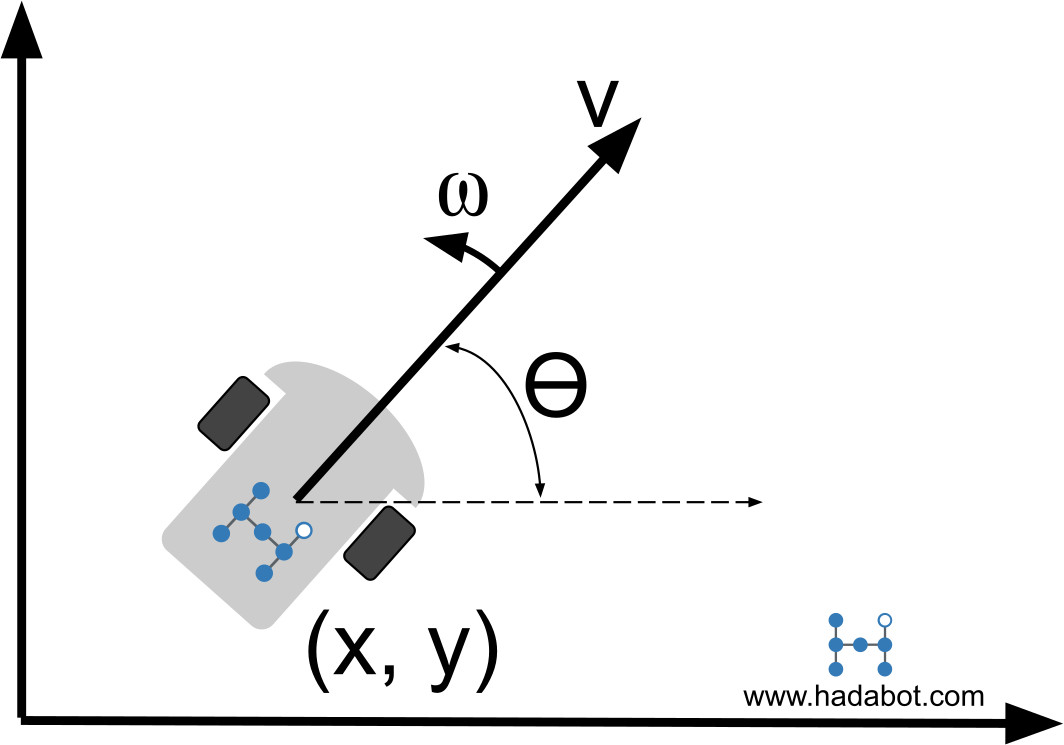
\includegraphics[width=\linewidth]{hadabot_unicycle_diagram_01.jpg}
	\caption{Graphical representation of 2D robot pose information standard to 2 wheel robots \cite{RN109}.}
\end{figure}
Our team's primary objective was to design a networked swarm of rovers capable of collaborative mapping, obstacle avoidance, and cooperative task execution. Our aim is to establish a foundational system that aids in Search and Rescue operations and facilitates research in multi-swarm rover technology. Presently, we've achieved success in creating rovers equipped with mapping capabilities, allowing real-time simultaneous visualization of surrounding areas within a simulation Moreover, our accomplishment includes developing these rovers at an affordable price point, under \$100 each. This cost-efficient solution stands in contrast to market offerings that typically start at \$300 for a turtle bot with a Jetson nano and increase steeply thereafter.

\section{Background} 
A plethora of elements must come together to successfully deploy a swarm of decentralized agents. Our system requires a working knowledge in both the physical and abstract. The agents are subject to their physical characteristics: i.e., their circuitry, power consumption, mechanical components, sensors, processing power, and geometry to navigate and respond to an environment. The complexity that drives cyber-physical systems is what largely makes robotics difficult. An agent must be able to function perfectly in a world with a continuous state space. Today, researchers are seeing a high degree of success with robots that incorporate mathematical and data driven modeling that leverages the superior computational capabilities of modern processors to solve complex continuous problems in robotics. 
\subsection{Common Robot Autonomous Platforms} Common mobile platforms for autonomous robots encompass a range of designs tailored to diverse applications within the field of robotics. Wheeled platforms, such as differential drive and omnidirectional robots, are popular choices due to their simplicity and efficiency in navigating various environments. Differential drive platforms use two powered wheels, allowing the robot to turn and move forward or backward by adjusting the speeds of the wheels. Omnidirectional platforms, on the other hand, utilize special wheel configurations to achieve unrestricted movement in any direction. Lastly, tracked platforms offer enhanced traction and stability, making them suitable for challenging terrains.

One notable platform is the TurtleBot 3, a popular open-source robot platform widely used for research and education. TurtleBot 3, developed by ROBOTIS, is a compact and modular robot equipped with various sensors, including a 360-degree lidar sensor, a camera, and inertial measurement units (IMUs). Its differential drive system allows for omnidirectional movement, making it versatile for navigation in dynamic environments. The TurtleBot 3 is often employed in the development and testing of autonomous navigation algorithms, mapping techniques, and obstacle avoidance strategies. Its affordability, ease of use, and vibrant community support make it an attractive choice for researchers, students, and hobbyists interested in exploring the intricacies of autonomous robotics.

\subsection{Robot Localization}
\begin{figure}
	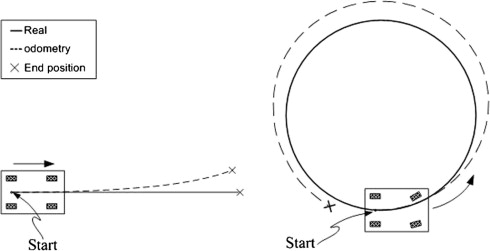
\includegraphics[width=\linewidth]{odometry_error.jpg}
	\caption{Graphical representation of basic odometry error as a robot follows a reference trajectory \cite{RN206}.}
\end{figure}
Normally, robots use a wide range of sensors to inform themselves about the surrounding environment. Our agents, for example, rely on a 6 axis inertial measurement unit (IMU) and rotatory encoders to produce an \{$X$, $Y$, $\theta$, $\dot{X}$, $\dot{Y}$, $\dot{\theta}$, $\ddot{X}$, $\ddot{Y}$\} state configuration at every time step by considering physical properties and mechanics (Fig. 1). However, a frequent problem with using rudimentary techniques solely for odometry is that error propagated at each time step due to environmental conditions, sensor specifications, electrical noise, and rounding error can deviate a naive agent during localization. The problem persists even with the use of a known map and highly accurate sensors. Consider how a human might traverse a city by using a map. The human could ensure their own position by simply pondering their place in respect to features of the map like buildings, intersections, or street signs. Even if the human absent mindlessly navigated the city, they could triangulate their location by simply calculating their positions based on observations (such as the coffee shop across the street). Our robots, incorporate a Kalman ExFor an agent, SLAM leverages known knowledge of poses at past time steps and emissions or observations (sensor readings) made as the agent accumulates error through basic odometry to calculate probabilities of where the agent can be in space. Any number of sensors that detect 'emissions' from the environment can be used for SLAM; however, 2D lidar and cameras are regularly used for the high degree of precision awarded. Agents are capable of both learning a new environment and updating a known map with SLAM; thus, justifying our deployment of SLAM to improve the navigation capabilities of each agent.

\subsection{Robot Kinematics} <Jordy>

\subsection{ROS2 and Open Source Frameworks} <Jordy>

\subsection{Robot Description and Transformation Trees} <Jordy>

\subsection{Gazebo for Robot Simulation} <Jordy>

\subsection{Autonomous Navigation} <Jordy>

\subsection{Multi-Agent Swarm Systems} <Jordy>

\section{Project Implementation}
\subsection{Preliminary Robot Chassis}

Our rover is designed with two distinct levels, both 3D-printed boards with holes to screw in different components. The upper level features the LiDAR for a clear view, with the wires going through the center of the 3D-printed board.
On the lower level, our lithium batteries are securely attached using Velcro at the rear. The power board is positioned at the front, fastened by two of the four poles securing both levels.
Beneath the bottom board,  two TT motors are firmly fixed to the 3D-printed board using screws, alongside encoders secured with a hot glue gun adjacent to the motors. Wires from the encoders, motors, and LiDAR are routed towards the rear, adjacent to the batteries, and connected to our power board. This central hub houses vital components such as the ESP32-wroom, IMU, and H-bridge.

The two levels are connected using 3D-printed poles, approximately 1½" in length. Additionally, a roller ball bearing is positioned at the rover's front, crucial for even weight distribution and smoother turns. Its absence previously caused calibration errors as the rover rocked back and forth during testing.


\subsection{Preliminary Electronics Design and Testing}
One of the hardware considerations is what board will run the rover firmware. Luckily, the choice of using ROS2 and Mircoros narrowed the choices down substantially. Microros provides a list of supported development boards. These boards range from Arduino, STM32, and Teenys to ESP32. Looking through the list of specific boards, it quickly became apparent that many were out of the budget. To give an idea, the two cheapest boards are the Raspberry Pi Pico (averages a cost of 6 dollars) and the ESP32-DevKitC-32UE/E (10 dollars). While the next cheapest board is the Teensy 4.1, which clocks in at about 30 dollars per board (a heavy price increase). With the choice coming down to either the Pi Pico or the ESP32, the final choice is ESP32 since it has WiFi built within the chip and is an entirely new option for experimenting. ESP32 developers, Espressif, drivers for I2C, UART, PWM, and ADC. These drivers are essential for interfacing with the sensor to determine pose.

For the rovers to fully function, they must take advantage of odometry, kinematics, and PID. To handle these calculations, the feedback/data from wheel movement and inertial acceleration allows for deriving the rover's pose. The infrared rotary encoder provides feedback to determine the speed of each motor, handling PID, and parts of odometry/kinematics. DAOKI offers a Slotted Optical IR encoder that is within the budget and a part that attaches itself to the TT motors for easier reading of motor speed. Although this encoder provides feedback, it is not enough to accurately determine the rover's pose, which is why the MPU 6050 gives us additional information for deriving the accuracy of its movement by measuring inertial acceleration. Between the MPU6050 and the DAOKI encoder's pose, odometry, kinematics, and PID are accurate enough to serve the parameters of the project. Now, concerning SLAM we could stick with just those two sensors, but the mapping and location would not be satisfactorily accurate without a lidar sensor. Our rovers feature the LiDAR HLS-LFCD2, LiDAR, an acronym for Light Detection and Ranging, utilizes light pulses to gauge distances from its location. To interface with the LiDAR, we use a serial connection to the microcontroller, where data received undergoes conversion to extract ranges and intensities. The processed data are then transformed into Laser Scan messages and relayed to the host computer. On the host side, this information serves as pivotal input for simulating a detailed map reflecting the rover's surroundings. This simulation acts as an invaluable debugging resource, ensuring alignment between the rover's real-world operations and the expected functionality within the simulated environment.

Testing for the hardware and sensors is divided into three steps: reference projects, ESP driver development, and testing on the ESP32 themselves. The first step for testing all sensors was finding projects/tutorials online. These tutorials offer a path to narrow down what parts of the datasheet are necessary for our interaction with the sensors. One example is the MPU6050 tutorial showing which addresses are relevant for XYZ gyro acceleration, setup for MPU before reading from those registers, along the math needed to be on the data to determine its angle. Many of these tutorials were in Arduino and meant for either the UNO or PI Pico, which the team had on hand from previous classes/projects, making the preliminary testing of seeing if the components were not defective a simple process. The next step is reshaping the tutorials into C using the Espressif drivers. Once refactored, the code is tested on the component again to ensure functionality is the same as the original testing, the new code is adjusted to fit the needs of Linorobot.





\subsection{Preliminary ROS2 Robot Description Design and Simulation}

\subsection{Hardware/Firmware}
Linorobot is the skeleton for the hardware of our little rovers. We attempted to use the original code built on Arduino and PlatformIO, but the project started with the team developing drivers on the Espressif IDF. The issue, however, is Arduino did not have any official documentation on the supported Espressif libraries/boards. A lack of documentation and not understanding Linorobot2 on how to change/add in our drivers left us with a decision. Dive deeper into and translate the drivers into Arduino/C++ or translate the main.c file along with kinematics, odometry, and PID over to Espressif/C and make sure our drivers follow a similar structure to Linorobot’s drivers in terms of formatting Microros data. Ultimately, the team found it easier to bring over the skeleton of Linorobot than to redo the drivers.

 For interacting with the MPU6050, the communication protocol is I2C. The setup for the MPU is simple; a zero byte is written to the power management register before data is to be read. After writing the zero bytes, the next step is measuring the error. We are only concerned with the GyroZ register. To calculate the error, while the MPU is still and data is being sampled multiple times, the average is taken to know how much drift there is within the system. The next time the register is read, we subtract that error from the reading to get an accurate value. It is also important to note that the value read must first be divided by 131 according to the datasheet to convert the value to scale.
 
 Encoder interactions only require counting pulses. Essentially, the encoders only have three pins: power, ground, and out. Out is either high or low on whether an object is blocking the IR sensor(in our case rotary attachments to the TT Motors). To achieve RPM calculations, use a PCNT(pulse counter) peripheral to count the rising edges of the Out pin outputs. Then it is a simple problem of using the number of pulses recorded since the last sample divided by the time since the last sample (dx/dt) and converting it to an RPM. For the DAKOI attachment, twenty triggerings of the sensor represent a full rotation.
 
 Analog-digital conversions did not require too much setup, mostly calibration steps were required from the Espressif. Very little needed to be changed from the example code keeping in the relevant calibration sequence chosen, which was a linear fitting. The ADC was used to detect battery voltage; sampling was done at a voltage divider since the ADC could only do a maximum of about 3V. If the sample was less than or equal to 2 V, the overall voltage of the battery was low, and continuing usage resulted in damage to the components.

The TT Motors were bought via Amazon and arrived approximately a week after ordering, priced at approximately \$6 per motor. Upon arrival, a visual inspection ensured there were no visible defects. Each motor featured a white rod on both ends, creating a T-shaped appearance, facilitating attachment of the wheel on one side and an encoder on the other to track rotations.
The initial functionality test involved connecting the red wire to 5 volts and the black wire to ground, which verified proper operation for all motors. Subsequently, assessing compatibility between the microcontroller, h-bridge, and the motors involved validating directional control for forward, backward, and turning movements. Manipulating speed required utilizing PWM within the Espressif framework, which posed challenges in integrating their new PWM drivers. After encountering multiple issues, a pivot to their older PWM driver ensued, demonstrating immediate functionality and seamless integration into the primary rover code.

Our rovers are equipped with the LiDAR HLS-LFCD2, utilizing a usart-based serial connection. Procured from eBay at an approximate cost of \$40 per unit, arriving in about one month. Upon arrival, our initial objective was to validate their functionality.
To verify functionality, we meticulously followed the instructions provided by Matthew Hogan's tutorial in \"Interesting Electronic Components \#1: HLS-LFCD2.\" This guided us through the process of interfacing the LiDAR with a Raspberry Pico, utilizing the Arduino IDE. This comprehensive procedure spanned nearly a month, involving debugging of provided code and checking hardware. Ultimately, the successful operation allowed us to generate x and y data points.
Having verified functionality, our focus shifted towards transitioning the system's programming from C++ to C and migrating to the Espressif framework instead of the Raspberry Pico. This strategic shift was a necessity as we are utilizing ESP32-wroom as our microcontroller for each rover.

After extensive refactoring from the Linorobot2 package, and overcoming several challenges, we achieved successful data publication from the lidar to our local host. This data facilitated real-time simulation, enabling mapping of the rover's surroundings. This accomplishment allowed us to showcase a live demonstration during our scheduled demo day.




\subsection{Multi-Agent Implementation with ROS2}

\section{Evaluation}
The IR encoders served their purpose to a usable level. The encoders can determine an RPM for PID and speed control, but with only 20 slots/encoder counts, the readings are most likely not entirely accurate. For the project and with the budget constraints they satisfy our needs. An experiment for future use is to 3D print a new attachment for the rotary piece with more slotted holes. However, issues to look out for in the future for testing more holes are whether the IR sensor can keep up / differentiate the smaller holes and whether the PCNT peripheral is able to keep up with counting the rising edges of the triggers.

For the IMU/MPU6050, the evaluation will fall under the same umbrella as the rotary encoders. It served the purpose of telling us the pose, but it came at the cost of drift to the point the host machine would struggle to understand/run simulations on the data being recieved. The host machine filters data to help with these issues, but it was not prepared to handle how much the data drifted from the MPU 6050. As for the reason why the data was not as good as it should have been, we have one theory. When developing the driver for the MPU6050, the steps taken in reading the data and applying math to the data are almost the same, with the only significant difference being the I2C driver reading data. When running the Arduino example code there is no major drift issue, which leads us to believe that the MPU6050 is to run on a microcontroller like the UNO as opposed to one such as the ESP32 deployed in the project. When checking the error value calculated between the two boards, the values from the UNO are closer to the one reported in the tutorial than the value from the ESP32. To figure out this issue, the first step that needs testing is trying complex calibration sequences as opposed to the simple ones used by both the tutorial and Linorobot. If the different calibration sequences do not work out, the next best option is to use the MPU9050. The reason for recommending the MPU9050 as opposed to the 6050 is the Espressif example tutorial for I2C uses MPU9050 and most likely supports it better than the 6050. Meaning the MPU6050 is reliable within the Arduino framework. However, switching to the 9050 is difficult due to budgeting constraints. With the 6050 a set of 5 costs about 10 dollars, while a single 9050 is about 12 dollars.

How effective was the LiDAR for our team? Its functionality met our project requirements by successfully extracting information from the LiDAR and transmitting it as messages to the host computer. We achieved mapping of the rover's surroundings at intervals of 1 second. For our specific project objectives, it fulfilled its designated tasks precisely and efficiently.

Regarding the performance of the Old PWM Driver, it efficiently regulated motor speed by managing the duty cycle. Implementing this older driver proved simpler compared to adopting the newer PWM library within Espressif.

As for the USART pins on the microcontroller, they functioned suitably for transmission and reception of data from the LiDAR. However, improved documentation would have been beneficial, as the process involved a considerable amount of trial and error to identify which USART pins were available for our purposes.


\section{Conclusion}
Microros for the ESP32 is an interesting situation. There is no doubt that the project would not have come together without the use of ROS2 and Microros. There is plenty of documentation on the tools/API and it supports the ESP32. The main trouble the team ran into was figuring out which information was relevant to the project and determining. Most of the issues encountered were either a miss-step in the step or interaction with the Microros variables and function calls. Once an understanding of what is needed, the tools act accordingly.

\section{Discoveries and Pitfalls}  
During the refactoring from Arudino/C++ to Espressif/C, the Microros libraries for Arduino are surprisingly very similar, and the developers did well at keeping the name of function calls to Macros and functionality. Unfortunately, there are differences that need mentioning. In the Arduino Microros, runtime variables do not need to be initialized, but in the Espressif and C it is required before use. Here is an example where in Arduino you would only need the second line, but in C you need the two:

\begingroup
\fontsize{5.70pt}{10pt}\selectfont
\begin{verbatim}  
	rosidl_runtime_c__String__init(odom_msg_.child_frame_id));
	odom_msg_.child_frame_id = 
	micro_ros_string_utilities_set(odom_msg_.child_frame_id, "base_footprint");  
\end{verbatim}  
\endgroup

Another example is the pinging of the Microros agent. In the original Linorobot's state machine states are Wait for Agent, Agent available, Agent Connected, and Agent Disconnected. We found that in the state Wait for the Agent, struggles to ping the host machine agent and gets stuck in that state. When that state is removed and goes straight for Agent Connected, the code is executed without issue. A delay is also placed in the Agent Connected so that the Watchdog timer does not trigger when the rover is idle for long periods. The last pitfall with Microros that the team discovered was the limitation with nodes.

 ROS and Microros allow Nodes to have multiple publishers and subscribers, but the Microros library for ESP32 has the default max for using nodes to one node, two subscribers, and two publishers. Luckily, these are not hard-set max values and require you to go to the library’s colcon.meta file to change the max value then clean/recompile the library.
 
An unexpected pitfall encounter was with the WiFi router used in the project. Essentially, the firewall on the router would block the microcontroller from initializing a ROS network if the controller is reset more than three times. To circumvent this issue, power cycle the router or turn off the firewall on the router. Turning off the firewall allowed for multiple resets of the board, but it still can/will get stuck with initializing the network if done too often.
 
Refactoring the lidar code base from C++ to C posed significant challenges, primarily due to the use of a different microcontroller with an entirely distinct framework. While working on the Pico, the capability to read a single byte at a time was feasible. However, transitioning to the Espressif framework posed a problem as it inherently reads multiple bytes, lacking the option to read singular bytes using USART. Also, identifying available USART pins on the microcontroller involved substantial trial and error. However, implementing the lidar onto the microcontroller presented numerous difficulties. The initial challenge surfaced as a watchdog warning during the first trial, triggered because the main system lacked resources to oversee its overall functionality, attributable to a while loop that didn't stop. The remedy involved incorporating a delay of 5 ticks at the end of the loop, to allow the system to check it’s status.

Subsequently, encounter issues while retrieving the complete stack of data from the lidar became apparent. Although we were receiving information from the serial line, our code expected the first byte read was the start of the frame, which was consistent only when starting the LiDAR to send data. After a while, the alignment in data we were reading was inconsistent. The solution to ensure consistent data framing,was to forcefully sending the character 'b', which is used to start sending data to the microcontroller. This was called in the polling method within our code, please refere to Appendix A line 1.

Further complexity arose when attempting to publish lidar data to our local host computer. It was able to publish data in it’s own project folder, however integration into our primary project file alongside other components resulted in the system to fail. The underlying issue stemmed from microROS, which imposed a limit on node creation set by a configuration file. After extensive research lasting 2-3 weeks, the solution emerged: modifying the configuration file.

\clearpage
\section{Appendices}
\begin{center}APPENDIX A
\end{center}
\begin{center}Inside the Lidar Polling Method
\end{center}
\begin{lstlisting}[frame=leftline, breaklines=true, numbers=left, stepnumber=1, numbersep=5pt]
error_tx = uart_write(test_str);


while(!successful_scan){
    uart_read_size = uart_read(data);
        
    if(uart_read_size > 0){
        sync[0] = data[0];
        sync[1] = data[1];
    }
    
    //First capture the start byte of a frame:
    //Once start byte captured, read remaining frame into array:
    if (sync[0] == 0xFA && sync[1] == 0xA0) {
        frame[0] = 0xFA;
        frame[1] = 0xA0;
        for (int v = 2; v <= 2520; v++) {
            frame[v] = data[v]; //copying the data from data array to frame
        }
        ready = true;
    }  
    
    //Once frame captured, extract range/angle and convert to x/y:
    if (ready) {
        lidar_msg_->angle_increment = (2.0*M_PI/360.0);
        lidar_msg_->angle_min = 0.0;
        lidar_msg_->angle_max = 2.0 * M_PI - lidar_msg_->angle_increment;
        lidar_msg_->range_min = 0.12;
        lidar_msg_->range_max = 3.5;
        
        for (uint16_t i = 0; i < 2520; i = i + 42) {
            if (frame[i] == 0xFA && frame[(i + 1)] == 0xA0 + (i / 42)) {                    
                good_sets++;
                motor_speed += (frame[i+3] << 8) + frame[i+2]; //accumlate count for avg. time increment
                for (uint16_t j = i + 4; j < i + 40; j = j + 6) {
                
                    index = 6*(i/42) + (j-4-i)/6;

                    uint8_t rangeA = frame[j + 2];
                    uint8_t rangeB = frame[j + 3];
                    uint8_t rangeC = frame[j];
                    uint8_t rangeD = frame[j+1];

                    uint16_t range = (rangeB << 8) + rangeA;
                    uint16_t intensity = (rangeD << 8) + rangeC; 

                    lidar_msg_->ranges.data[359-index] = range/1000.0;
                    lidar_msg_->intensities.data[359-index] = intensity;
                }
            }
        }
        
        rpms = motor_speed / good_sets / 10;
        lidar_msg_->time_increment = (float)(1.0 / (rpms*6));
        lidar_msg_->scan_time = lidar_msg_->time_increment * 360;

        ready = false;
        num_of_times_it_made_it++;
        successful_scan = true;
    }  
    else {
        sync[0] = 0;
        sync[1] = 0;
        did_not_work++;
        }

    if(did_not_work >= 5 )
    {
        num_reset++;
        ESP_LOGI(TAG_LIDAR, "Number of resets of lidar: %d\n Current value of conversions: %d", num_reset, num_of_times_it_made_it);
        vTaskDelay(5);
        free(data);
        return false;                      
    }
}

free(data);
return successful_scan;

\end{lstlisting}

\nocite{*}
\bibliographystyle{ieeetran}
\bibliography{citations}% Produces the bibliography via BibTeX.
\vspace{12pt}

\end{document}